\documentclass[journal,12pt,twocolumn]{article}
\usepackage[top = 1in,bottom = 1in,left = 1in,right = 1in]{geometry}
\setlength{\columnsep}{2cm}
\usepackage{amssymb}
\usepackage{amsfonts}
\usepackage{amsmath}
\usepackage{amsthm}
\usepackage{setspace}
\usepackage{longtable}
\usepackage{enumitem}
\usepackage{mathtools}
\usepackage{color}                                  
\usepackage{array}
\usepackage{calc} 
\usepackage{bm}
\usepackage{caption}
\usepackage{float}
%has mini page
%to fix position (H)

\setlength{\parindent}{0pt}
%no indentation for paragraphs

\begin{document}

\title{ASSIGNMENT-3}
\author{MUKUNDA REDDY AI21BTECH11021}
\date{}
\maketitle
\section*{Exercise 16.3}
\textbf{17)} A and B are events such that ${P(A) = 0.42}$, ${P(B) = 0.48}$ and
${\text{P(A and B)} = 0.16}$. Determine\\
 (i)  P(not A)\\
(ii)  P(not B) \\
(iii) P(A or B) \\
\hline

\section*{Solution}
\subsection*{(i) Determine p(not A)}
Given $P(A) = 0.42$ so we have
\begin{align*}
    P(\overline{A}) &= 1 - P(A)\\ 
                    &= 1 - 0.42\\   
                    &= 0.58 
\end{align*}
\begin{equation}
 \therefore P(not A) = 0.58    
\end{equation}

\begin{figure}[H]
    \centering
    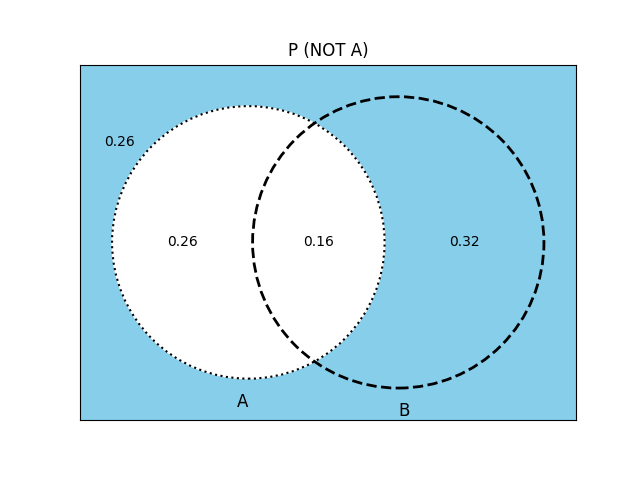
\includegraphics[scale=0.5]{Figure_1.png}
    \caption{P(\overline{A})}
    \label{fig:1}
\end{figure}


\subsection*{(ii) Determine p(not B)}
Given $P(B) = 0.48$ so we have
\begin{align*}
    P(\overline{B}) &= 1 - P(B)\\ 
                    &= 1 - 0.48\\   
                    &= 0.52
\end{align*}
\begin{equation}
 \therefore P(not \ B) = 0.52   
\end{equation}
\begin{figure}[H]
    \centering
    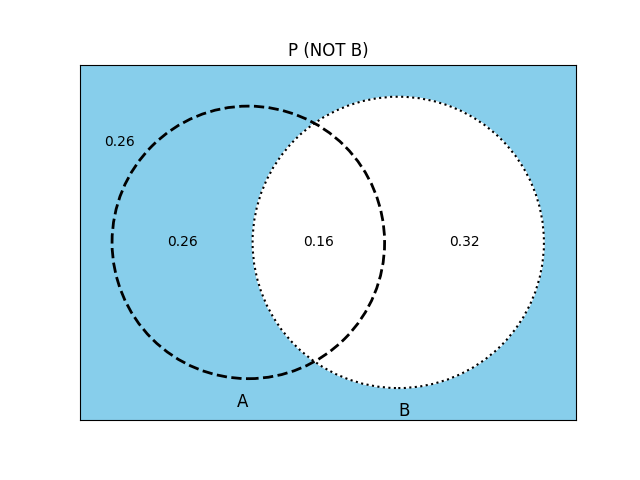
\includegraphics[scale=0.5]{Figure_2.png}
    \caption{P(\overline{B})}
    \label{fig:2}
\end{figure}

\subsection*{(iii) Determine p(A or B)}
Given ${P(A\cap\ B) = 0.16}$,${P(A) = 0.42}$ \\
${P(B) =0.48}$ so we have\\
\begin{align*}
    P(A \cup\ B) &=P(A) + P(B) - P(A \cap\ B) \\
                &= 0.42 + 0.48 - 0.16 \\ 
                &= 0.74 \\
\end{align*}
\begin{equation}
 \therefore P(A\ or \ B) = 0.74  
\end{equation}
\begin{figure}[H]
    \centering
    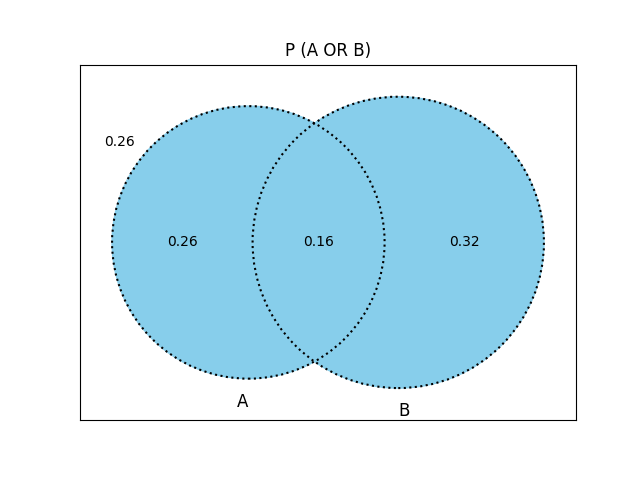
\includegraphics[scale=0.5]{Figure_3.png}
    \caption{P(A \cup\ B)}
    \label{fig:3}
\end{figure}


\section*{Verification}

\begin{figure}[H]
    \centering
    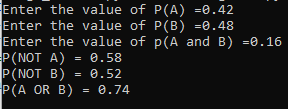
\includegraphics[scale=1]{Figure_4.png}
    \caption{python code}
    \label{fig:4}
\end{figure}

\end{document}
